% informe.tex - Documentación sobre el trabajo práctico para entregar

\documentclass{article}
\usepackage[utf8]{inputenc}
\usepackage[spanish]{babel}
\usepackage{graphicx}

\begin{document}

\title{Informe Trabajo Práctico 1}
\author{Victoria Perelló (89608)\\
        \and
        Agustín Mezzina (89637)\\
	\and
        Pablo Rodríguez (93970)}
\maketitle

\section{Procesos}
La aplicación se divide en los siguientes procesos:
\begin{enumerate}
	\item Init: llena la cola de autos entrantes.
	\item Jefe de estación: recibe los autos entrantes y los asigna a empleados libres. En caso de no haber empleados libres, los despacha.
	\item Empleado: asigna autos a surtidores libres. Si no hay surtidores libres, espera a que se libere alguno. Realiza el servicio. Cobra y guarda la recaudación en la caja.
	\item Consulta caja registradora: consulta asincrónica sobre el valor de la recaudación en caja.
\end{enumerate}

\section{Comunicación entre procesos}
En el siguiente diagrama, se muestra el esquema de comunicación entre los procesos del sistema. Incluye los datos que intercambian los procesos que se comunican entre sí y los recursos a los que deben acceder de manera concurrente.
\\[1\baselineskip]
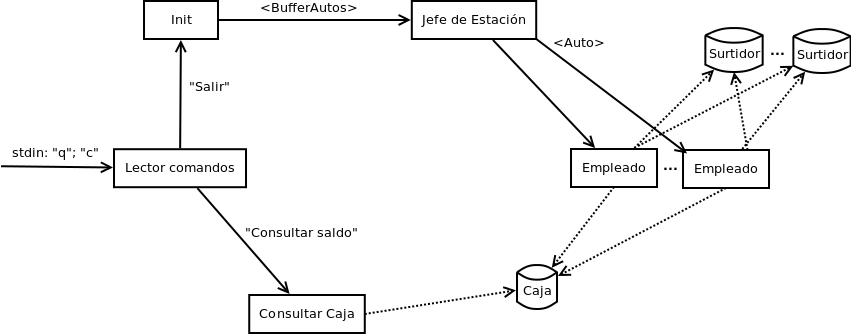
\includegraphics[width=\textwidth]{overview}

\section{Problemas conocidos de concurrencia}
\begin{enumerate}
	\item Init - Jefe de estación: Productor - Consumidor. El proceso base hace las veces de Productor, ingresando autos nuevos a un buffer compartido donde posteriormente el Jefe de Estación, en este caso Consumidor, los retira según su orden de llegada y los procesa.
	\item Jefe de estación - Empleado(s): Sección Crítica y Productor - Consumidor. El problema de la Sección Crítica se da cuando los procesos se comuniquen su respectiva disponibilidad para poder trabajar. El problema del Productor - Consumidor aparece con la espera de los Empleados de un Auto de parte del Jefe para que el mismo pueda ser atendido.
	\item Empleado - Empleado: Sección Crítica. Los procesos deben excluirse mutuamente al ejecutar código que acceda a los recursos Surtidores.
	\item Empleado(s) - Consultar Caja: Sección Crítica. Los procesos deben excluirse mutuamente al ejecutar código que acceda al recurso Caja.
\end{enumerate}
\section{Mecanismos de concurrencia a utilizar}
En el siguiente diagrama se muestran los mecanismos de concurrencia utilizados para lograr la comunicación y sincronización de procesos:
\\[1\baselineskip]
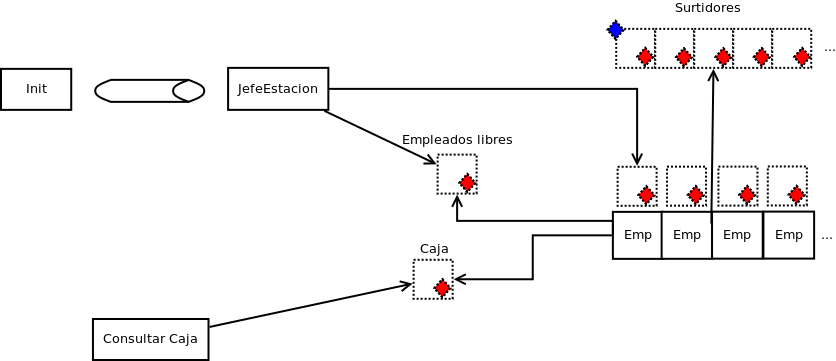
\includegraphics[width=\textwidth]{mecanismos}
\subsection{Init - Jefe de estación}
El buffer de autos se implementó utilizando un named pipe (o FIFO), de manera que el proceso inicial ingresa los autos al canal a medida que los va produciendo y el jefe de estación los toma en orden para procesarlos. Este mecanismo de concurrencia provee no sólo comunicación entre ambos procesos, sino que también sincronismo.
\subsection{Jefe de estación - Empleado(s)}
Los procesos tienen un espacio de memoria compartida donde se guarda el dato de cuántos empleados libres hay en la estación. Si este número es igual a 0, el jefe de estación descarta el auto que está atendiendo. Si no lo es, decrementa en valor en 1 y asigna el auto a uno de los empleados libres. Cuando el empleado termina de trabajar con el auto y se libera, aumenta el valor de la variable. Esta memoria compartida está protegida con un semáforo.
Además cada Empleado mantiene con el Jefe de Estación otro espacio de memoria compartida, cada uno también protegido con un semáforo, donde se intercambia información sobre el estado del Empleado y se guarda el auto que debe ser atendido.
\subsection{Empleado - Empleado}
Los Surtidores están guardados en bloques de memoria compartida accesibles a todos los Empleados. Dicho bloque está protegido por un semáforo general que permite el acceso al área de memoria cuando haya algún surtidor libre. Cada espacio de memoria donde se encuentra un surtidor está, a su vez, protegido por un semáforo binario.
\subsection{Empleado(s) - Consultar Caja}
Estos procesos acceden a un espacio de memoria compartida donde está la Caja. Dicho espacio está protegido por un semáforo para resolver el problema de sección crítica que se da cuando algún proceso quiera ingresar o extraer dinero de ella.

\end{document}
